% !TEX program = pdflatex
%
% Financial Econometrics - Homework 5
% Two-page report: Dynamic Conditional Correlations during financial turmoil.
% Companion code & dashboard: https://github.com/tamaradokic/Financial-Econometrics-HW5-

\documentclass[a4paper,9pt,twocolumn]{extarticle}

\usepackage[margin=1.3cm,columnsep=0.55cm]{geometry}
\usepackage{graphicx}
\usepackage{booktabs}
\usepackage{amsmath}
\usepackage{amssymb}
\usepackage{xcolor}
\usepackage{hyperref}
\usepackage{caption}
\usepackage{titlesec}
\usepackage{microtype}
\usepackage{makecell}

\hypersetup{colorlinks=true,urlcolor=blue!45!black,linkcolor=black,citecolor=black}
\captionsetup{font=small,labelfont=bf,skip=3pt,labelsep=period}
\titleformat{\section}{\normalsize\bfseries}{\thesection.}{0.5em}{}
\titlespacing*{\section}{0pt}{6pt}{2pt}
\setlength{\parskip}{0.25\baselineskip}
\setlength{\parindent}{0pt}
\setlength{\abovedisplayskip}{3pt}
\setlength{\belowdisplayskip}{3pt}
\setlength{\abovedisplayshortskip}{2pt}
\setlength{\belowdisplayshortskip}{2pt}

\title{\vspace{-1.4cm}\textbf{Dynamic Conditional Correlations during financial turmoil}\\[2pt]
  \normalsize Financial Econometrics, Homework 5 \\
  \small ESSEC Master in Data Science \& Business Analytics, term T3 2025--26}
\author{\small Tamara Dokic \,\textbar\, Valentin Levy \,\textbar\, Baptiste Noel \,\textbar\, Sagar Vishishta}
\date{\vspace{-6pt}\small \today}

\pagestyle{empty}

\begin{document}
\twocolumn[%
  \begin{@twocolumnfalse}
    \maketitle
    \vspace{-1.2em}
    \begin{abstract}\noindent\small
      We estimate a multivariate DCC--GARCH(1,1) model on five sector-diverse US equities (NVIDIA, Tesla, Eli~Lilly, JPMorgan Chase, ExxonMobil) over 2016--2026 and apply the model's time-varying covariance matrix to construct a minimum-variance portfolio (MVP). The DCC dynamics uncover substantial intertemporal variation in pairwise correlations; \textbf{9 of 10 pairs exhibit sign reversals}, a pattern that the unconditional correlation matrix entirely conceals. The DCC-based MVP delivers a strictly lower realized variance than the static-covariance MVP, providing direct empirical support for modelling time-variation in the second moments. The naive equal-weighted (1/$N$) portfolio nonetheless attains the highest realized Sharpe ratio, reproducing the well-known result of DeMiguel, Garlappi, and Uppal (2009) on the difficulty of beating naive diversification.
    \end{abstract}
    \vspace{0.6em}
  \end{@twocolumnfalse}
]

\section{Data}
Daily adjusted closing prices for NVDA, TSLA, LLY, JPM, XOM were retrieved from Yahoo Finance for the period 2016-06-14 to 2026-06-11 ($T = 2{,}513$ trading days). Returns are continuously compounded percentage log differences, $r_{i,t} = 100\log(P_{i,t}/P_{i,t-1})$. The universe spans semiconductors/AI, automotive/EV, pharmaceuticals, banking and energy, sectors with distinct macroeconomic drivers and therefore plausibly time-varying co-movement.

\textbf{Stylized facts.} All five series display pronounced leptokurtosis (sample excess kurtosis up to $13.6$ for JPM), strong rejection of normality by the Jarque--Bera test, and highly significant ARCH effects (Engle's ARCH--LM$(10)$ $p$-value $<10^{-3}$ in every case). These two stylized facts, fat tails and conditional heteroskedasticity, motivate the GARCH framework used throughout.

\section{Methodology}
We follow Engle's (2002) two-step DCC procedure.

\textbf{Step 1: univariate GARCH.} For each asset $i$,
\begin{equation*}
r_{i,t} = \mu_i + \varepsilon_{i,t}, \quad \varepsilon_{i,t} = \sigma_{i,t} z_{i,t},
\end{equation*}
\begin{equation*}
\sigma_{i,t}^2 = \omega_i + \alpha_i\varepsilon_{i,t-1}^2 + \beta_i\sigma_{i,t-1}^2,
\end{equation*}
with $z_{i,t} \sim \mathcal{N}(0,1)$. The five fitted persistences $\hat\alpha_i + \hat\beta_i$ lie between $0.93$ and $0.998$, in the textbook range for daily equity volatility.

\textbf{Step 2: DCC.} On the standardized residuals $z_{i,t} = \varepsilon_{i,t}/\sigma_{i,t}$,
\begin{equation*}
Q_t = (1-a-b)\,\bar Q + a\, z_{t-1} z_{t-1}^{\top} + b\, Q_{t-1},
\end{equation*}
\begin{equation*}
R_t = \mathrm{diag}(Q_t)^{-1/2}\, Q_t\, \mathrm{diag}(Q_t)^{-1/2},
\end{equation*}
where $\bar Q$ is the sample covariance of $z_t$ (correlation targeting). The two scalar parameters $(a,b)$ are estimated by Gaussian quasi-MLE on the composite likelihood under the stationarity constraints $a\geq 0$, $b\geq 0$, $a+b<1$. The full conditional covariance is $\Sigma_t = D_t R_t D_t$, with $D_t = \mathrm{diag}(\sigma_{1,t},\ldots,\sigma_{N,t})$.

\section{Estimation results}
The DCC parameter estimates are
\[
\hat a = 0.022,\quad \hat b = 0.958,\quad \hat a + \hat b = 0.980,
\]
with composite log-likelihood $743.78$. The persistence is high but strictly less than one, satisfying covariance stationarity: correlation shocks dissipate gradually, producing regimes that persist for many months.

\textbf{Dynamic correlations (Figure~\ref{fig:rho}).} The DCC uncovers dependence structures that the unconditional matrix entirely obscures. \textbf{Nine of the ten unique pairs flip sign} at some point in the sample, transitioning between regimes of positive and negative co-movement. The widest range is the JPM--XOM pair, whose conditional correlation varies from $-0.07$ to $+0.70$. All pairs exhibit sharp upward movements during the COVID-19 shock of March~2020 and during the 2022 monetary tightening cycle, the empirical signature of \textit{financial contagion}. The practical implication is that the diversification benefit available from any given asset pair is itself state-dependent and tends to deteriorate precisely when it would be most valuable.

\begin{figure*}[t]
\centering
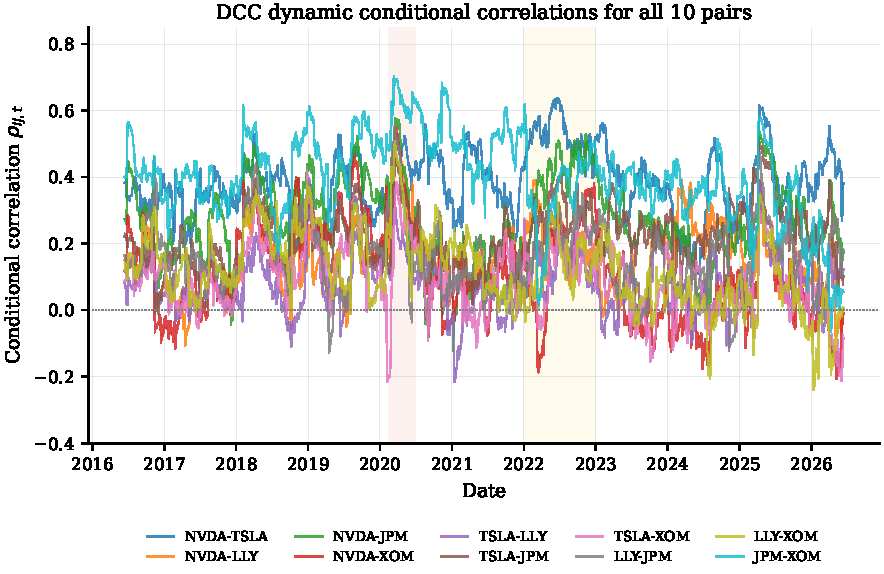
\includegraphics[width=0.97\textwidth]{figures/fig_correlations.pdf}
\caption{Dynamic conditional correlations $\rho_{ij,t}$ for all ten unique asset pairs, estimated by DCC--GARCH(1,1). Shaded bands mark the COVID-19 episode (Feb--Jun 2020) and the 2022 monetary tightening cycle. Nine of ten pairs exhibit sign reversals; JPM--XOM has the widest range, $[-0.07,\, 0.70]$.}
\label{fig:rho}
\end{figure*}

\section{Portfolio construction}
The closed-form minimum-variance allocation is
\begin{equation*}
w_t^* = \frac{\Sigma_t^{-1}\mathbf{1}}{\mathbf{1}^{\top}\Sigma_t^{-1}\mathbf{1}}.
\end{equation*}
Substituting the DCC-implied $\Sigma_t$ yields a dynamic MVP that rebalances every day; substituting the unconditional sample covariance $\hat\Sigma$ instead yields the classical Markowitz (1952) static MVP, with one allocation vector applied uniformly across the sample. We also benchmark against the naive equal-weighted (1/$N$) portfolio. Portfolio returns use \emph{lagged} weights, $r_{p,t} = w_{t-1}^{\top} r_t$, to preclude look-ahead bias.

\textbf{Average allocations.} The DCC-MVP holds, on average, $\{3.5\%, 3.4\%, 27.8\%, 31.5\%, 33.7\%\}$ across $\{$NVDA, TSLA, LLY, JPM, XOM$\}$, concentrating in the lower-volatility assets. The static MVP allocates similarly on average but cannot adapt to crisis-period changes in $\Sigma_t$. Figure~\ref{fig:weights} contrasts the dynamic weight trajectories with the static benchmark.

\begin{figure}[t]
\centering
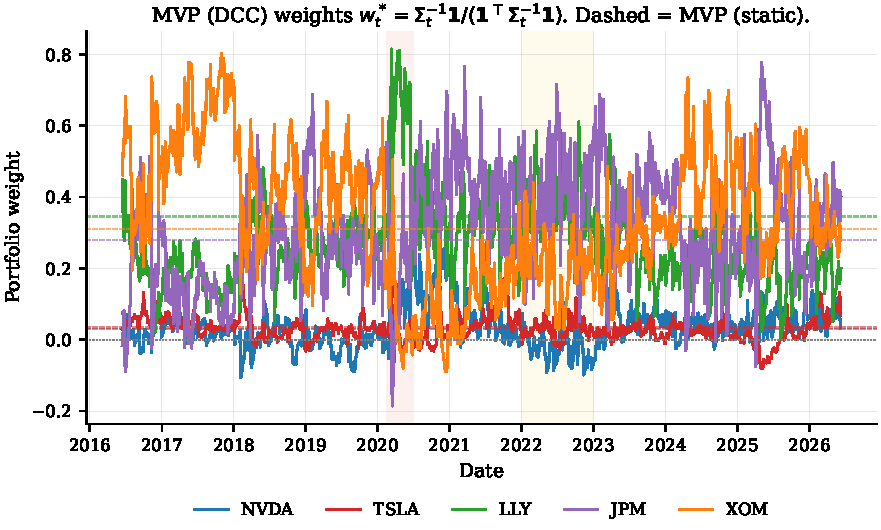
\includegraphics[width=\linewidth]{figures/fig_weights.pdf}
\caption{Time series of MVP (DCC) weights $w_t^*$ (solid lines). Dashed horizontal lines show the corresponding MVP (static) allocations, identical at every date. The gap between solid and dashed measures how strongly the dynamic model deviates from the static benchmark; the largest deviations occur during the crisis episodes shaded in the background.}
\label{fig:weights}
\end{figure}

\section{Empirical performance and verdict}
Table~\ref{tab:perf} reports the realized full-sample performance of the three strategies. Sharpe ratios are computed against the 3-month US Treasury bill yield (FRED series \texttt{DGS3MO}), the academic-convention proxy for the risk-free rate; the sample-average yield is $2.40\%$, materially above zero and concentrated in 2023--2025.

\begin{table}[h]
\centering\small
\begin{tabular}{lrrr}
\toprule
Strategy & \makecell[r]{Ann.\ Ret.\\(\%)} & \makecell[r]{Ann.\ Vol.\\(\%)} & \makecell[r]{Sharpe\\(rf=2.4\%)} \\
\midrule
MVP (DCC)    & 19.79 & 20.09 & 0.865 \\
MVP (static) & 20.96 & 20.64 & 0.899 \\
Equal-weight (1/$N$) & \textbf{28.52} & 25.41 & \textbf{1.028} \\
\bottomrule
\end{tabular}
\caption{Realized portfolio performance, full sample. Sharpe ratio computed with the time-varying 3M T-bill yield (DGS3MO, sample mean $2.40\%$).}
\label{tab:perf}
\end{table}

\begin{figure}[h]
\centering
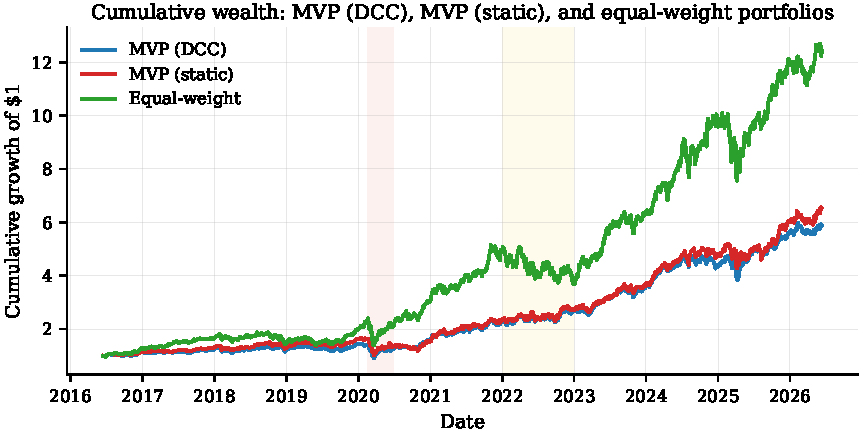
\includegraphics[width=\linewidth]{figures/fig_cumret.pdf}
\caption{Cumulative growth of \$1, gross of transaction costs, applying lagged weights to daily returns.}
\label{fig:cumret}
\end{figure}

Two findings stand out.

\textbf{(i) The DCC dynamics are empirically valuable.} The DCC-MVP attains a strictly lower realized variance ($1.602$ vs $1.690$ per day, a $5.2\%$ reduction) than the static MVP. This is direct empirical evidence that incorporating time-variation in $\Sigma_t$ produces genuine risk reduction rather than spurious in-sample fit: if the dynamics were noise, the two strategies would be statistically indistinguishable.

\textbf{(ii) Equal-weighting is hard to beat on Sharpe.} The 1/$N$ portfolio attains a Sharpe ratio of $1.028$, materially above both optimization-based strategies. The driver is the higher annualized return ($28.5\%$ vs $20$--$21\%$): the DCC- and static-MVPs underweight the high-mean, high-volatility assets (NVDA, TSLA) that drove most of the sample's equity returns. This reproduces the celebrated DeMiguel--Garlappi--Uppal (2009) finding that estimation error in the covariance matrix penalizes optimization-based portfolios out-of-sample relative to the naive benchmark.

\textbf{Which strategy to invest in?} The answer is preference-dependent. For a variance-minimizing investor (e.g.\ a pension fund near maturity), the DCC-MVP is the rational choice: it delivers the lowest realized risk. For a return-maximizing investor with tolerance for higher volatility and estimation error, the equal-weight strategy historically outperforms on risk-adjusted terms. The fundamental contribution of the DCC framework is to make the first option \textit{empirically improvable} on top of static Markowitz; the choice between the dynamic MVP and 1/$N$ then becomes a statement about the investor's objective function, not about model fit.

\vspace{4pt}
\rule{\linewidth}{0.3pt}
\footnotesize
\textbf{Code and interactive dashboard.} All source code, the eight-question Streamlit dashboard with interactive DCC parameter what-if sliders and a custom-portfolio comparator, and this report are available upon request.


\end{document}
